\documentclass[aspectratio=169,10pt]{beamer}

% ---------------------------------------------------------------------------
% Paquetes
% ---------------------------------------------------------------------------
\usepackage[utf8]{inputenc}
\usepackage[T1]{fontenc}
\usepackage{lmodern}
\usepackage{graphicx}
\usepackage{booktabs}
\usepackage{array}
\usepackage{enumitem}
\usepackage{tikz}
\usepackage{pgfplots}
\pgfplotsset{compat=1.17}
\usetikzlibrary{arrows.meta,positioning,shapes.geometric}

% ---------------------------------------------------------------------------
% Paleta de colores (navy / azul)
% ---------------------------------------------------------------------------
\definecolor{navy}{RGB}{16,32,63}
\definecolor{steel}{RGB}{43,92,157}
\definecolor{steellight}{RGB}{140,175,214}
\definecolor{bgpanel}{RGB}{240,243,247}
\definecolor{graytext}{RGB}{95,95,95}

% ---------------------------------------------------------------------------
% Tema base minimalista
% ---------------------------------------------------------------------------
\usetheme{default}
\setbeamertemplate{navigation symbols}{}
\setbeamertemplate{headline}{}

\setbeamercolor{normal text}{fg=black,bg=white}
\setbeamercolor{structure}{fg=navy}
\setbeamercolor{title}{fg=white,bg=navy}
\setbeamercolor{frametitle}{fg=navy,bg=white}
\setbeamercolor{alerted text}{fg=steel}
\setbeamercolor{block title}{fg=white,bg=steel}
\setbeamercolor{block body}{fg=black,bg=bgpanel}
\setbeamercolor{itemize item}{fg=steel}
\setbeamercolor{itemize subitem}{fg=steellight}
\setbeamerfont{frametitle}{series=\bfseries}
\setbeamerfont{footline}{size=\scriptsize}

\setbeamertemplate{itemize item}{\raise1.2pt\hbox{\textcolor{steel}{\rule{4pt}{4pt}}}}
\setbeamertemplate{itemize subitem}{\raise1.2pt\hbox{\textcolor{steellight}{\rule{3pt}{3pt}}}}

\setlist[itemize]{itemsep=5pt, topsep=3pt, leftmargin=*}
\setlist[itemize,2]{itemsep=3pt, topsep=2pt}
\setlist[enumerate]{itemsep=5pt, topsep=3pt, leftmargin=*}

% Título de frame minimalista con regla inferior
\setbeamertemplate{frametitle}{
  \vspace{4pt}
  \hspace{2pt}\textcolor{navy}{\Large\bfseries\insertframetitle}\par
  \vspace{2pt}
  \hspace{2pt}\textcolor{steel}{\rule{0.94\paperwidth}{0.7pt}}
  \vspace{6pt}
}

% Footer: solo numeración de página, sin autor/fecha/navegación
\setbeamertemplate{footline}{
  \hfill
  \raisebox{6pt}{\textcolor{graytext}{\scriptsize\insertframenumber\,/\,\inserttotalframenumber}}
  \hspace{10pt}
  \vspace{6pt}
}

\setbeamertemplate{blocks}[rounded][shadow=false]

% Comando auxiliar para notas de fuente al pie de una figura
\newcommand{\fuente}[1]{\vspace{2pt}\textcolor{graytext}{\scriptsize #1}}

\title{Impactos de la educación parvularia pública en Chile en fertilidad y mercado laboral de las madres}
\author{Micaella Magnasco}
\date{Julio 2026}

\begin{document}

% =============================================================================
% 1. PORTADA
% =============================================================================
\begin{frame}[plain]
\vspace{50pt}
\begin{center}
{\LARGE\bfseries\color{navy} Impactos de la educación parvularia pública\\[3pt] en Chile en fertilidad y mercado laboral\\[3pt] de las madres}

\vspace{10pt}
\textcolor{steel}{\rule{0.5\paperwidth}{0.6pt}}

\vspace{14pt}
{\large\color{graytext} Estado de avance del proyecto de tesis}

\vspace{55pt}
{\normalsize
Micaella Magnasco \\[4pt]
\small Profesor guía: Andrés Hojman \\[2pt]
\small Actividad Final de Grado --- Pontificia Universidad Católica de Chile \\[2pt]
\small Julio 2026
}
\end{center}
\end{frame}

% =============================================================================
% 2. MOTIVACIÓN
% =============================================================================
\begin{frame}{Motivación}
\begin{itemize}
  \item En el \textbf{96\,\%} de los hogares con menores de 7 años, la madre ejerce el rol de cuidadora principal (MDSF, 2017); las mujeres destinan el doble de horas diarias que los hombres al cuidado (MDSF, 2023).
  \item Esta carga de cuidados limita la inserción laboral femenina y condiciona las decisiones reproductivas.
  \item La participación laboral femenina se mantiene estancada en torno al \textbf{50\,\%}, y la tasa de fertilidad ha caído a \textbf{1,17 hijos por mujer}, una de las más bajas del mundo (OCDE, 2025).
  \item Cerca de \textbf{150.000 mujeres} que salieron de la fuerza laboral durante la pandemia aún no han regresado, especialmente madres con hijos menores de 5 años.
  \item El tema es central en el debate legislativo actual: \textbf{Ley de Sala Cuna Universal} (en tramitación en el Senado) y \textbf{Ley Chile Cuida / SNAC} (promulgada en febrero de 2026), que crea el cuidado como cuarto pilar de la protección social.
\end{itemize}
\end{frame}

% =============================================================================
% 3. PREGUNTA DE INVESTIGACIÓN Y OBJETIVOS
% =============================================================================
\begin{frame}{Pregunta de investigación y objetivos}
\begin{block}{Pregunta de investigación}
\small ¿Cuáles son los efectos de la expansión pública de la educación parvularia en Chile sobre la participación laboral femenina y la fertilidad de las madres?
\end{block}

\vspace{6pt}
\begin{block}{Objetivo general}
\small Estimar el efecto causal de la apertura de jardines infantiles públicos (JUNJI/Integra) sobre la participación laboral y la fertilidad de las madres, explotando la variación territorial y temporal de su expansión escalonada entre 2016 y 2023.
\end{block}
\end{frame}

% =============================================================================
% 4. CONTEXTO — GOBERNANZA Y PROVISIÓN MIXTA
% =============================================================================
\begin{frame}{Educación parvularia en Chile: gobernanza y provisión}
\begin{columns}[T]
\begin{column}{0.52\textwidth}
\begin{itemize}
  \small
  \item \textbf{Subsecretaría de Educación Parvularia} (Mineduc): diseño, coordinación y gestión de política. Desde la reforma de 2015, separada de la provisión directa.
  \item \textbf{Provisión pública}: JUNJI y Fundación Integra (salas cuna y jardines, foco en hogares vulnerables) + provisión municipal (NT1--NT2, vía subvención escolar).
  \item \textbf{Provisión privada}: particulares subvencionados y particulares pagados, con mayor peso en zonas urbanas y niveles de transición.
  \item Sistema de \textbf{gobernanza centralizada y provisión mixta}.
\end{itemize}
\end{column}
\begin{column}{0.44\textwidth}
\small
\begin{table}
\begin{tabular}{@{}lr@{}}
\toprule
\textbf{Tipo de establecimiento} & \textbf{\%} \\
\midrule
Particulares subvencionados & 34,7 \\
JUNJI AD y VTF & 26,5 \\
Escuelas municipales & 20,1 \\
Integra AD y CAD & 10,3 \\
Escuelas SLEP & 4,3 \\
Particulares pagados & 3,5 \\
Jardines privados & 0,6 \\
\bottomrule
\end{tabular}
\end{table}
\vspace{4pt}
{\small\textbf{61,2\,\% pública} \textbar\ \textbf{38,8\,\% privada} (2024)}
\fuente{Fuente: Informe de caracterización de la Educación Parvularia 2024, SdEP.}
\end{column}
\end{columns}
\end{frame}

% =============================================================================
% 5. CONTEXTO — COBERTURA ACTUAL Y BRECHAS
% =============================================================================
\begin{frame}{Cobertura actual y brechas}
\begin{itemize}
  \item La asistencia neta a educación parvularia (0--5 años) sube de \textasciitilde50\,\% (2015) a \textbf{55\,\%} (2024), tras una caída marcada en pandemia (41\,\% en 2020) \small{--- Fuente: Centro de Estudios Mineduc, Encuesta CASEN.}
  \item Solo el \textbf{23\,\%} de los niños y niñas en edad de \textbf{sala cuna (0 a 2 años)} asiste a un establecimiento, muy por debajo del promedio OCDE (\textbf{85\,\%}), pese a una inversión superior al promedio de la organización.
  \item Fuerte gradiente socioeconómico: la asistencia es considerablemente mayor en los quintiles superiores (OCDE, 2025; Bronfman y Buitrago, 2021).
  \item Persisten \textbf{brechas territoriales} en la expansión reciente --- la sección de cobertura de este avance profundiza en su distribución regional.
\end{itemize}
\vspace{10pt}
\begin{block}{En síntesis}
\small A pesar de la expansión sostenida desde los años 90, la cobertura pública sigue siendo insuficiente y desigual, lo que motiva estudiar sus efectos causales sobre las decisiones de las madres.
\end{block}
\end{frame}

% =============================================================================
% 6. CONTEXTO — EVOLUCIÓN HISTÓRICA
% =============================================================================
\begin{frame}{Evolución histórica: contexto y período de estudio}
\begin{itemize}
  \small
  \item Antes de 2015, la oferta pública se expande gradualmente: creación de JUNJI (\textbf{1970}), Programa Educativo Alternativo de los años 90, meta de 120 mil cupos del gobierno de Lagos, Programa VTF (\textbf{2006}) y la Ley General de Educación (\textbf{2009}), que formaliza el nivel.
  \item Este trabajo se concentra en \textbf{2015--2024}: es el período para el cual JUNJI e Integra entregaron registros administrativos completos y georreferenciados, y coincide con la ventana de apertura escalonada de jardines (2016--2023) usada para la identificación.
\end{itemize}

\vspace{10pt}
\begin{block}{El período de estudio en cifras}
\small Más de \textbf{700 nuevos jardines públicos} JUNJI + Integra entre 2015 y 2024; la oferta pasa de 3.729 a 4.432 centros (\textbf{+19\,\%}), con expansión más acelerada entre 2015 y 2019 y desaceleración posterior a la pandemia.
\end{block}
\end{frame}

% =============================================================================
% 7. IDENTIFICACIÓN — DISEÑO
% =============================================================================
\begin{frame}{Estrategia de identificación: diseño}
\begin{columns}[T]
\begin{column}{0.56\textwidth}
\begin{itemize}
  \small
  \item Diseño cuasi-experimental de \textbf{diferencias en diferencias con estudio de eventos (event study)}, con efectos fijos bidireccionales (TWFE) de unidad vecinal y año.
  \item \textbf{Unidad de análisis}: unidad vecinal (UV) --- subdivisión territorial de una comuna, creada para descentralizar la gestión comunitaria y promover la participación ciudadana. El MDS la usa para sectorizar el país, focalizar beneficios estatales y analizar datos del Registro Social de Hogares (RSH); ofrece mayor desagregación que la literatura comparada.
  \item \textbf{Tratamiento}: una UV se considera tratada desde el año en que se inaugura el primer jardín infantil público dentro de su territorio \emph{o en una UV contigua}, permaneciendo tratada el resto del período (tratamiento absorbente).
  \item Apertura escalonada entre \textbf{2016 y 2023} $\to$ variación territorial y temporal que identifica el efecto.
\end{itemize}
\end{column}
\begin{column}{0.4\textwidth}
\small
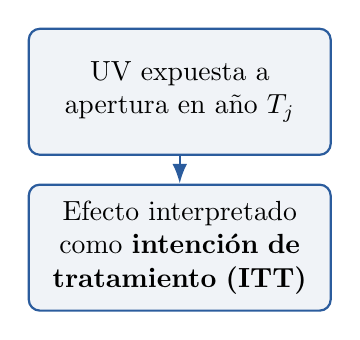
\begin{tikzpicture}
\node[draw=steel,thick,fill=bgpanel,rounded corners,text width=3.6cm,align=center,minimum height=1.6cm] (a) {UV expuesta a apertura en año $T_j$};
\node[draw=steel,thick,fill=bgpanel,rounded corners,text width=3.6cm,align=center,minimum height=1.6cm,below=10pt of a] (b) {Efecto interpretado como \textbf{intención de tratamiento (ITT)}};
\draw[-{Latex[length=2.5mm]},steel,thick] (a) -- (b);
\end{tikzpicture}
\vspace{6pt}

\small El efecto captura el impacto promedio de residir en un territorio con mayor \emph{acceso potencial} a educación parvularia pública, no la participación efectiva del hogar.
\end{column}
\end{columns}
\end{frame}

% =============================================================================
% 8. IDENTIFICACIÓN — ECUACIÓN DEL MODELO
% =============================================================================
\begin{frame}{Especificación empírica}
\[
Y_{ijt} = \lambda_j + \lambda_t + \sum_{k \neq -1} \beta_k \, \mathbb{1}\{t - T_j = k\} \, D_j + X'_{ijt}\gamma + \varepsilon_{ijt}
\]

\vspace{2pt}
\begingroup
\setlist[itemize]{itemsep=1pt,topsep=1pt,leftmargin=*}
\begin{itemize}
  \footnotesize
  \item $Y_{ijt}$: resultado del hogar $i$ en la UV $j$, año $t$. \quad $\lambda_j,\lambda_t$: efectos fijos de UV y año.
  \item $T_j$: año de apertura del primer jardín en la UV $j$; $k$ es el tiempo relativo a la apertura.
  \item $D_j$: indicador de UV alguna vez tratada. \quad $X_{ijt}$: controles a nivel de hogar.
  \item $\beta_k$: efecto ITT $k$ años antes/después de la apertura, respecto al período $t=-1$ (referencia).
\end{itemize}
\endgroup

\vspace{2pt}
\begin{block}{Coeficientes pre-apertura ($k<0$)}
\footnotesize deben ser estadísticamente indistinguibles de cero $\to$ evidencia de tendencias paralelas.
\end{block}

\vspace{1pt}
\footnotesize Dado que el tratamiento es escalonado, el TWFE estándar puede generar ponderaciones negativas al usar unidades ya tratadas como control. El \textbf{estimador exacto que corrige este problema aún no está definido}: se evaluarán alternativas (ETWFE, Wooldridge 2021; Callaway y Sant'Anna, 2021) según sus ventajas y desventajas.
\end{frame}

% =============================================================================
% 9. IDENTIFICACIÓN — SUPUESTOS Y AMENAZAS
% =============================================================================
\begin{frame}{Supuestos de identificación}
\begin{itemize}
  \item \textbf{Tendencias paralelas}: se evalúa con los coeficientes pre-apertura del event study; deben ser estadísticamente indistinguibles de cero.
  \item \textbf{No anticipación}: las madres no ajustan decisiones antes de la apertura efectiva. Su validez depende del grado de aviso previo con que se anuncian las aperturas (a analizar).
  \item \textbf{Exogeneidad del timing}: el momento de instalación no debe correlacionarse con características no observadas de la UV. \textbf{Principal amenaza}: que JUNJI/Integra prioricen unidades con mayor demanda de cuidado o características socioeconómicas particulares.
\end{itemize}

\vspace{10pt}
\begin{block}{Chequeo de plausibilidad (placebo)}
\small Se estimará un event study análogo usando la \textbf{tasa de natalidad pre-tratamiento} de la UV como variable de resultado. Coeficientes pre-tratamiento no significativos fortalecerían el supuesto de tendencias paralelas del modelo principal.
\end{block}
\end{frame}

% =============================================================================
% 10. COBERTURA — OBJETIVO (eje central de este avance)
% =============================================================================
\begin{frame}{La base de cobertura: eje central de este avance}
\begin{block}{Objetivo}
\small Construir un \textbf{panel balanceado a nivel de unidad vecinal (UV) $\times$ año} (6.877 UVs $\times$ 10 años, 2015--2024), donde cada fila indica cuántos centros de educación parvularia JUNJI e Integra existían en esa UV ese año.
\end{block}

\vspace{10pt}
\begin{itemize}
  \item Es la \textbf{pieza del proyecto completamente construida, verificada y documentada} hasta ahora (código, outputs y codebook en el repositorio).
  \item Define la variable de tratamiento a nivel de UV que se usará en el event study, y es el insumo territorial sobre el que se construirá el panel de resultados (mujer-UV).
  \item Las siguientes slides muestran cómo se construyó (pipeline) y sus cifras y gráficos principales.
\end{itemize}
\end{frame}

% =============================================================================
% 10b. COBERTURA — PIPELINE DE CONSTRUCCIÓN
% =============================================================================
\begin{frame}{Construcción de la base de cobertura: pipeline}
\begin{center}
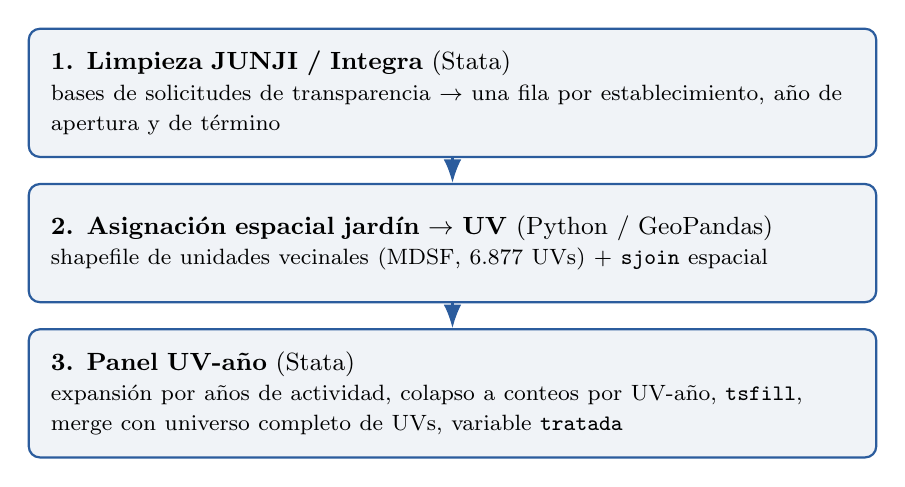
\begin{tikzpicture}[
  box/.style={draw=steel,thick,fill=bgpanel,rounded corners,text width=10.2cm,align=left,minimum height=1.5cm,inner sep=8pt,font=\small},
  arr/.style={-{Latex[length=3mm]},steel,thick}
]
\node[box] (b1) {\textbf{1. Limpieza JUNJI / Integra} (Stata) \\ \footnotesize bases de solicitudes de transparencia $\to$ una fila por establecimiento, año de apertura y de término};
\node[box, below=9pt of b1] (b2) {\textbf{2. Asignación espacial jardín $\to$ UV} (Python / GeoPandas) \\ \footnotesize shapefile de unidades vecinales (MDSF, 6.877 UVs) + \texttt{sjoin} espacial};
\node[box, below=9pt of b2] (b3) {\textbf{3. Panel UV-año} (Stata) \\ \footnotesize expansión por años de actividad, colapso a conteos por UV-año, \texttt{tsfill}, merge con universo completo de UVs, variable \texttt{tratada}};
\draw[arr] (b1) -- (b2);
\draw[arr] (b2) -- (b3);
\end{tikzpicture}
\end{center}
\vspace{4pt}
\fuente{Fuentes: solicitudes de transparencia JUNJI e Integra; shapefile de unidades vecinales, Ministerio de Desarrollo Social y Familia (BIDAT). Output final: \texttt{data/final/base\_cobertura\_cp.dta}.}
\end{frame}

% =============================================================================
% 11. COBERTURA — CIFRAS CLAVE
% =============================================================================
\begin{frame}{Base de cobertura: cifras clave}
\begin{itemize}
  \small
  \item Panel balanceado: \textbf{6.877 unidades vecinales $\times$ 10 años} (2015--2024) = \textbf{68.770 observaciones}.
  \item La oferta pública total pasó de \textbf{3.729 a 4.432 centros} entre 2015 y 2024 (\textbf{+19\,\%}); JUNJI concentra \textasciitilde74\,\% de los centros, Integra \textasciitilde26\,\%.
  \item \textbf{263 UVs} pasan de 0 a 1+ centros durante la ventana 2015--2024 (margen extensivo, variable \texttt{tratada}).
  \item El spatial join asignó UV al 100\,\% de los jardines con coordenadas válidas; quedaron fuera del panel \textbf{353 jardines JUNJI y 11 Integra} sin coordenadas utilizables.
\end{itemize}

\vspace{4pt}
\begin{block}{Nota metodológica}
\footnotesize La mayor parte de la expansión observada ocurre en el \textbf{margen intensivo} (UVs que ya tenían cobertura y suman más centros), no en el margen extensivo (UVs que pasan de 0 a 1+). Las \textasciitilde2.430 UVs que ya tenían cobertura en 2015 nunca pueden marcarse como \texttt{tratada}, por falta de datos previos a ese año.
\end{block}
\end{frame}

% =============================================================================
% 12. COBERTURA — EVOLUCIÓN JUNJI / INTEGRA (full bleed)
% =============================================================================
\begin{frame}{Evolución de la oferta pública, 2015--2024}
\begin{center}
\includegraphics[width=0.86\textwidth,height=0.76\textheight,keepaspectratio]{../output/figures/06_jardines_junji_integra_por_anio.png}
\end{center}
\fuente{Fuente: elaboración propia, \texttt{code/build/03\_panel\_uv\_anio.do} sobre \texttt{base\_cobertura\_cp.dta}.}
\end{frame}

% =============================================================================
% 13. COBERTURA — COMPOSICIÓN MODALIDADES JUNJI (full bleed)
% =============================================================================
\begin{frame}{Composición de jardines JUNJI por modalidad}
\begin{center}
\includegraphics[width=0.82\textwidth,height=0.74\textheight,keepaspectratio]{../output/figures/09_composicion_modalidades_junji.png}
\end{center}
\fuente{Fuente: elaboración propia sobre \texttt{base\_cobertura\_cp.dta}. Clásico Directo y Alternativo dominan la composición de JUNJI durante todo el período.}
\end{frame}

% =============================================================================
% 14. COBERTURA — COHORTES DE TRATAMIENTO POR AÑO
% =============================================================================
\begin{frame}{Cohortes de tratamiento por año}
\begin{center}
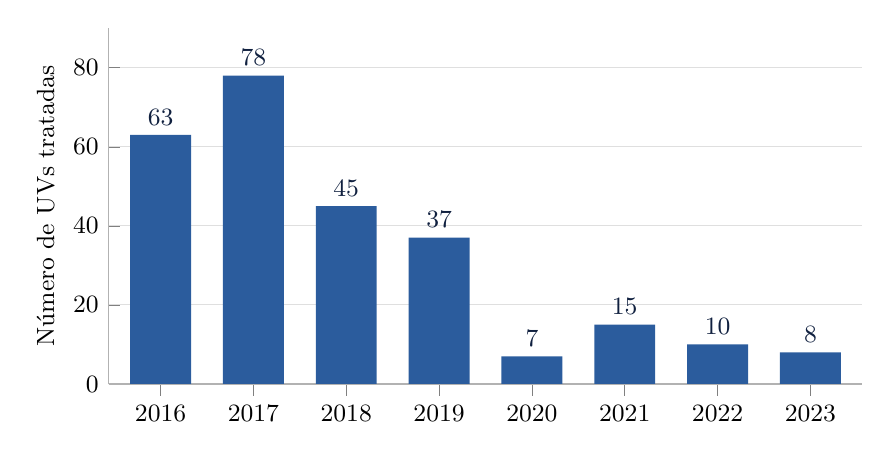
\begin{tikzpicture}
\begin{axis}[
  ybar,
  bar width=22pt,
  width=0.92\textwidth,
  height=6.1cm,
  symbolic x coords={2016,2017,2018,2019,2020,2021,2022,2023},
  xtick=data,
  ymin=0, ymax=90,
  nodes near coords,
  nodes near coords style={font=\small,text=navy},
  ylabel={N\'umero de UVs tratadas},
  ylabel style={font=\small},
  tick label style={font=\small},
  axis lines*=left,
  enlarge x limits=0.08,
  ymajorgrids=true,
  grid style={gray!25},
  axis line style={gray!60},
]
\addplot[fill=steel,draw=none] coordinates {
  (2016,63) (2017,78) (2018,45) (2019,37) (2020,7) (2021,15) (2022,10) (2023,8)
};
\end{axis}
\end{tikzpicture}
\end{center}
\vspace{2pt}
\small \textbf{263 UVs tratadas} en total (2016--2023). El 71\,\% (186 UVs) se concentra entre 2016 y 2018.
\fuente{Fuente: elaboración propia a partir de \texttt{base\_cobertura\_cp.dta} (\texttt{docs/codebook\_panel\_final.md}).}
\end{frame}

% =============================================================================
% 15. COBERTURA — MAPA JARDINES RM (full bleed)
% =============================================================================
\begin{frame}{Jardines públicos por unidad vecinal, Región Metropolitana}
\begin{center}
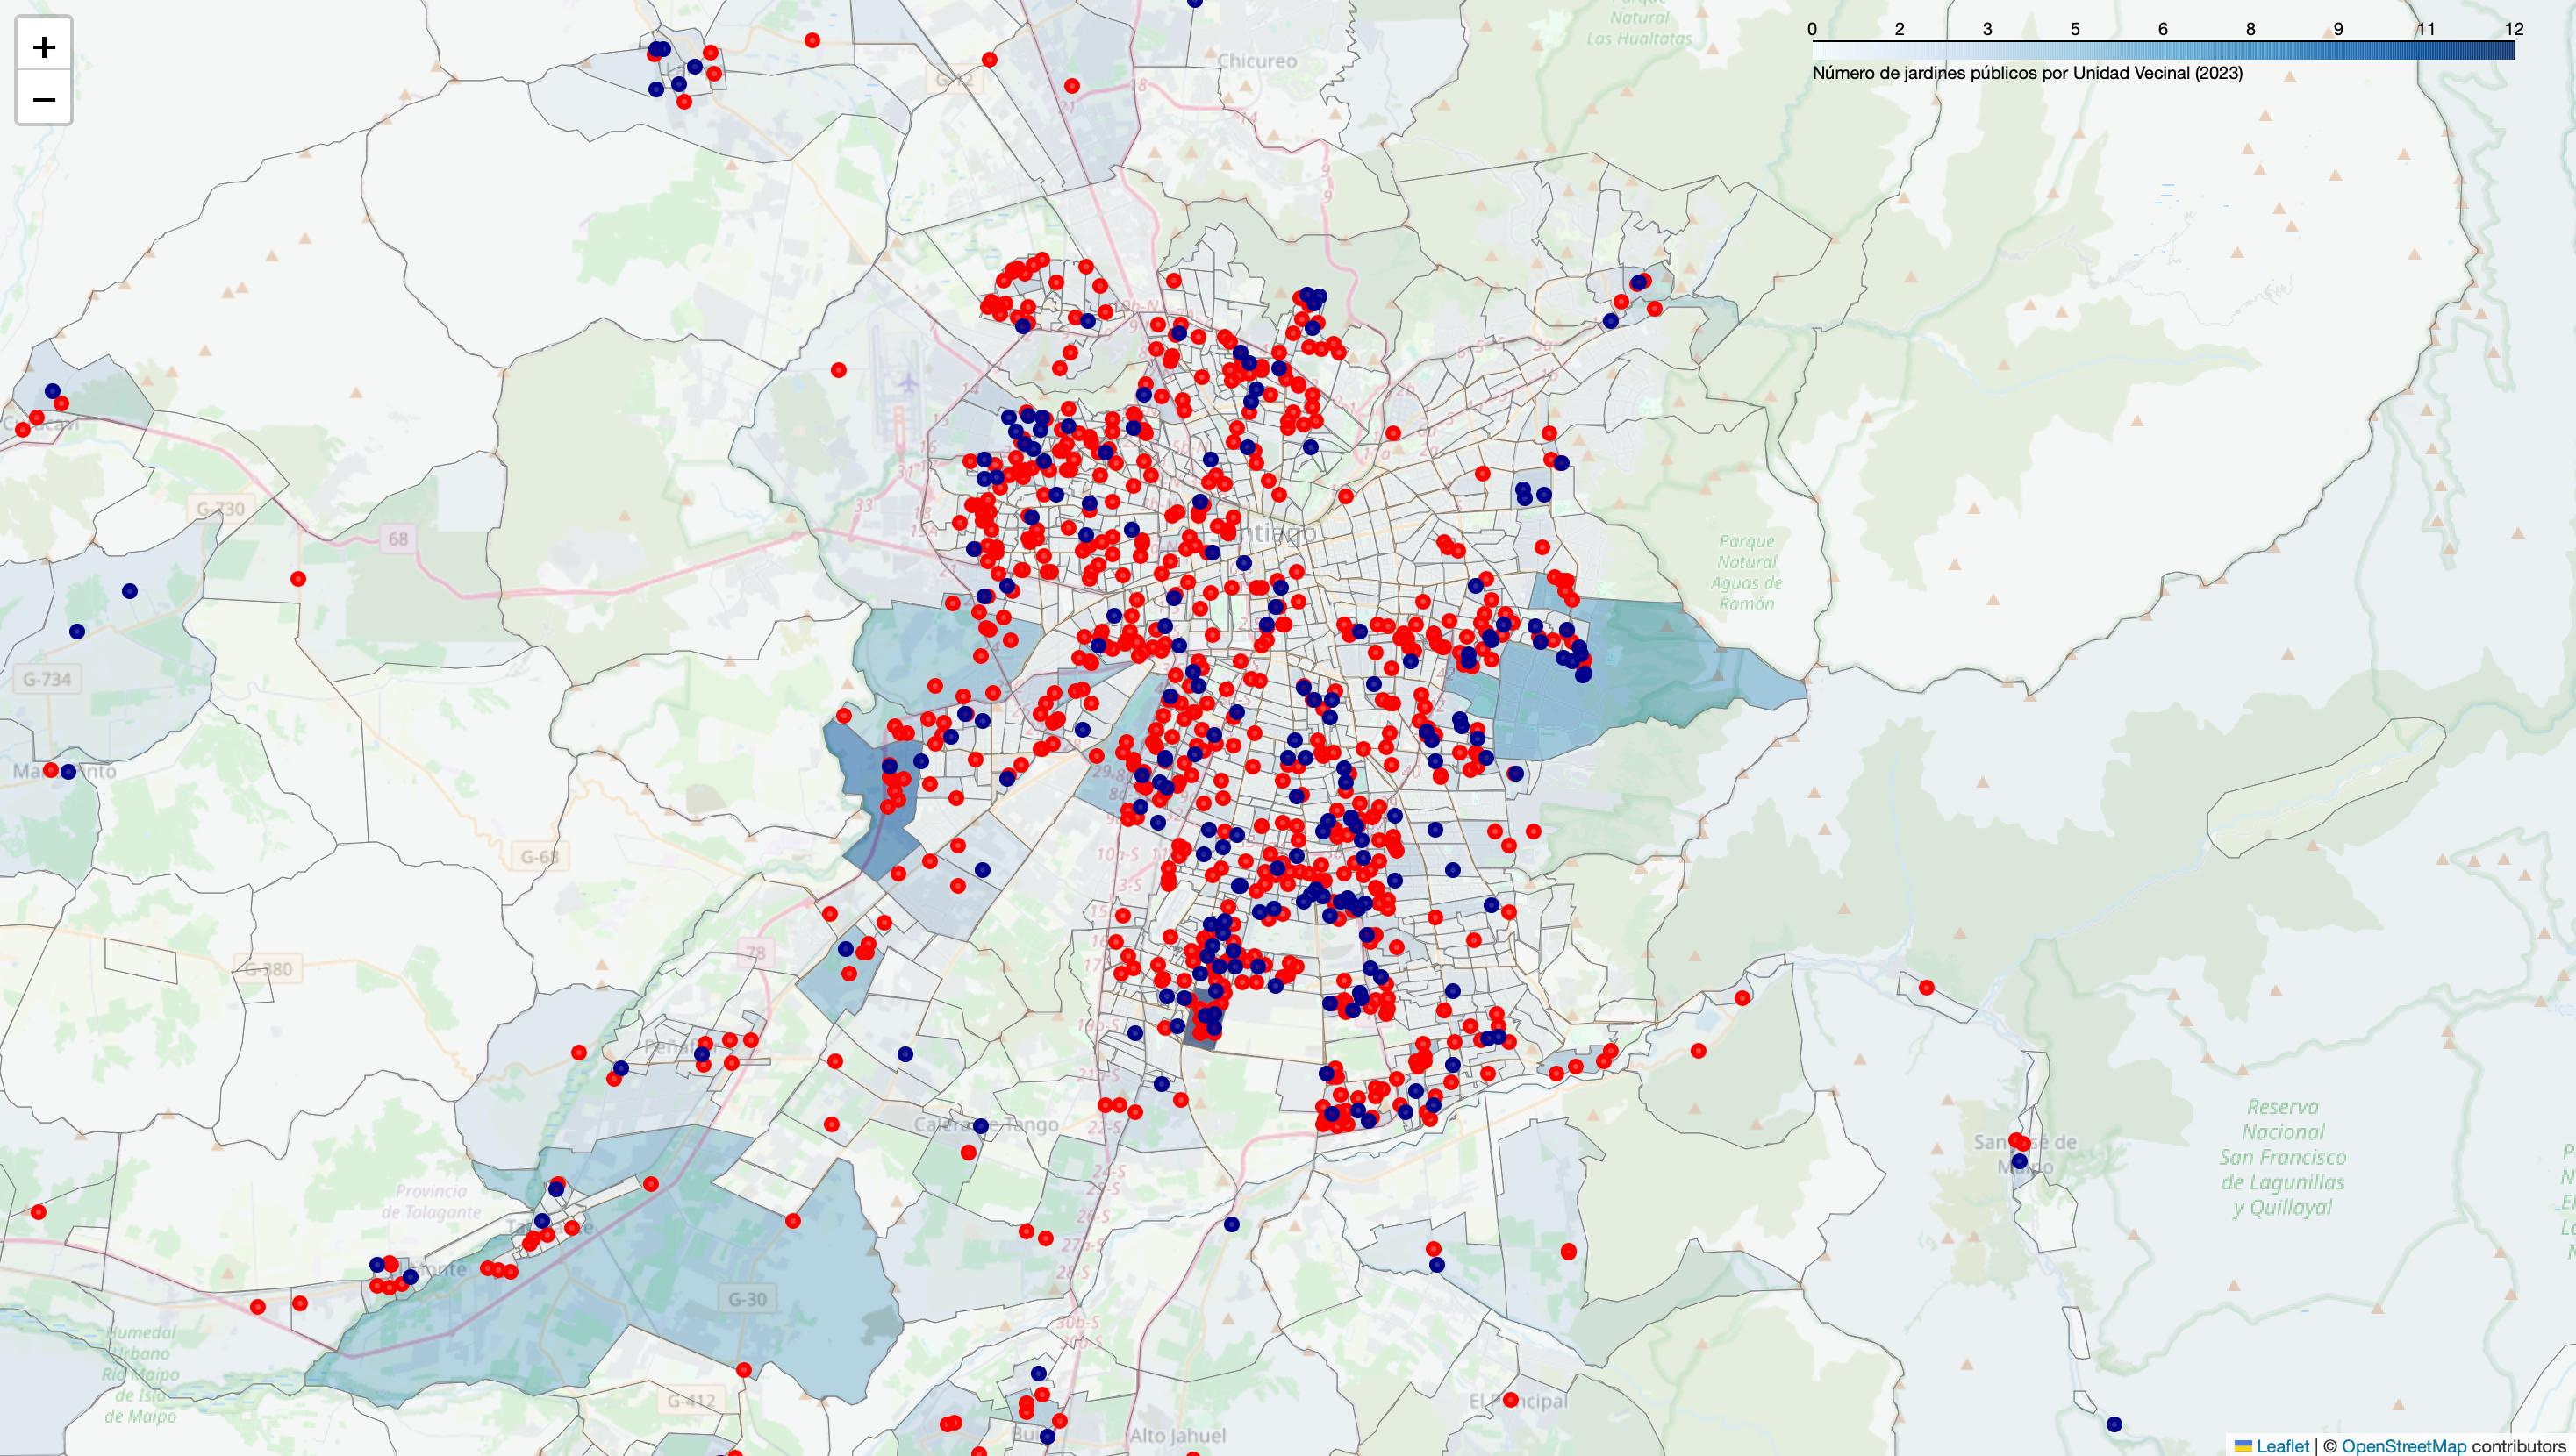
\includegraphics[width=0.92\textwidth,height=0.8\textheight,keepaspectratio]{../jardines_rm.jpeg}
\end{center}
\fuente{Fuente: elaboración propia a partir de \texttt{base\_cobertura\_cp.dta}. Puntos: jardines JUNJI (rojo) e Integra (azul); color de fondo: n\'umero de jardines p\'ublicos por UV (2023).}
\end{frame}

% =============================================================================
% 16. COBERTURA — DISTRIBUCIÓN TERRITORIAL Y CONCENTRACIÓN
% =============================================================================
\begin{frame}{Distribución territorial y concentración de la cobertura}
\begin{columns}[T]
\begin{column}{0.5\textwidth}
\centering
\includegraphics[width=\textwidth,height=0.62\textheight,keepaspectratio]{../output/figures/03_uv_tratadas_por_region.png}
\small Metropolitana (52) y Valparaíso (44) concentran el 37\,\% de las UVs tratadas.
\end{column}
\begin{column}{0.5\textwidth}
\centering
\includegraphics[width=\textwidth,height=0.62\textheight,keepaspectratio]{../output/figures/08_histograma_n_total_2024.png}
\small La mayoría de las UVs tiene 0 o 1 centro en 2024: distribución muy concentrada en el margen inferior.
\end{column}
\end{columns}
\fuente{Fuente: elaboración propia sobre \texttt{base\_cobertura\_cp.dta}, 2024.}
\end{frame}

% =============================================================================
% 17. COBERTURA — MAPA UVs TRATADAS (full bleed)
% =============================================================================
\begin{frame}{UVs tratadas: RM y Valparaíso (2015--2024)}
\vspace{-4pt}
\begin{columns}[T]
\begin{column}{0.5\textwidth}
\centering
\includegraphics[width=0.95\textwidth,height=0.64\textheight,keepaspectratio]{../output/figures/mapa_uv_tratadas_panel.png}
\end{column}
\begin{column}{0.5\textwidth}
\centering
\includegraphics[width=0.95\textwidth,height=0.64\textheight,keepaspectratio]{../output/figures/mapa_uv_tratadas_valparaiso.png}
\end{column}
\end{columns}
\fuente{Fuente: elaboración propia a partir de \texttt{base\_cobertura\_cp.dta}. UV tratada: pasa de 0 a 1+ jardines entre 2015 y 2024.}
\end{frame}

% =============================================================================
% 16. PANEL MUJER-UV — EN CONSTRUCCIÓN
% =============================================================================
\begin{frame}{Base de panel mujer--UV: en construcción}
\begin{block}{Objetivo del panel}
\footnotesize Construir un panel de \textbf{mujeres de 18 a 65 años} a partir del Registro Social de Hogares (RSH), con su \textbf{UV asignada}, que incorpore variables de \textbf{fertilidad} (si tuvo hijos en el período) y de \textbf{mercado laboral} (empleo, ingresos, entre otras).
\end{block}
\vspace{1pt}
\begingroup
\setlist[itemize]{itemsep=1pt,topsep=1pt,leftmargin=*}
\begin{columns}[T]
\begin{column}{0.5\textwidth}
{\footnotesize\textbf{Variables de mercado laboral}}
\begin{itemize}
  \footnotesize
  \item Rentas (bases ``Cuentas'', RUT innominado)
  \item Cotizaciones (Super\_Pensiones)
  \item Búsqueda de empleo / contrato (RSH)
\end{itemize}
\vspace{1pt}
{\footnotesize\textbf{Variables de fertilidad}}
\begin{itemize}
  \footnotesize
  \item Hijos vivos/fallecidos por RUT innominado
  \item Composición del hogar (RSH)
\end{itemize}
\end{column}
\begin{column}{0.5\textwidth}
{\footnotesize\textbf{Variables complementarias}}
\begin{itemize}
  \footnotesize
  \item Asignación de UV (RSH)
  \item Participación en educación parvularia de los hijos (RSH + SIMCE)
  \item Características territoriales de la UV
\end{itemize}
\vspace{1pt}
\begin{block}{Estado actual}
\footnotesize Ninguno de estos componentes tiene código terminado en el repositorio todavía. La \textbf{base de cobertura} (sección anterior) es, por ahora, la única etapa completamente construida y verificada.
\end{block}
\end{column}
\end{columns}
\endgroup
\end{frame}

% =============================================================================
% 17. PASOS A SEGUIR
% =============================================================================
\begin{frame}{Próximos pasos}
\begin{itemize}[label={}]
  \small
  \item \textbf{1.}~Terminar el panel \textbf{RSH-UV} (mujer-año) y el pipeline de \textbf{cotizaciones} (Super\_Pensiones).
  \item \textbf{2.}~Construir \textbf{características a nivel de UV} (variables territoriales/socioeconómicas para heterogeneidad y controles).
  \item \textbf{3.}~Extender y limpiar la \textbf{base de nacimientos}.
  \item \textbf{4.}~\textbf{Primer paso analítico}: validación de primera etapa --- event study de matrícula/asistencia a jardines centrado en el año de apertura de la UV.
  \item \textbf{5.}~Estimar efectos en \textbf{participación laboral} (rentas, cotizaciones, búsqueda de empleo) y en \textbf{fertilidad} (nacimientos).
  \item \textbf{6.}~\textbf{Robustez}: reestimar con el estimador de \textbf{Callaway y Sant'Anna (2021)} para tratamiento escalonado.
  \item \textbf{7.}~Placebo de exogeneidad del timing con tasa de natalidad pre-tratamiento.
\end{itemize}
\end{frame}

% =============================================================================
% 18. RESULTADOS PRINCIPALES
% =============================================================================
\begin{frame}{Resultados principales}
\vspace{20pt}
\begin{center}
{\Large\bfseries\color{navy} Resultados pendientes}
\end{center}
\vspace{18pt}

\begin{itemize}
  \item La base de cobertura (UV-año) está construida y verificada; la base de resultados (mujer-UV: RSH, cotizaciones, nacimientos) está en construcción.
  \item Aún no se han estimado modelos de participación laboral ni de fertilidad.
  \item El primer resultado esperado es la \textbf{validación de primera etapa} (matrícula/asistencia), seguido de las estimaciones de impacto descritas en ``Próximos pasos''.
\end{itemize}
\end{frame}

\end{document}
